\documentclass{article}
\usepackage[english]{babel}
\usepackage[T1]{fontenc}
\usepackage{wrapfig}
\usepackage{lscape}
\usepackage{rotating}
\usepackage{graphicx}
\usepackage{listings}
\usepackage{amsmath}
\usepackage{amsfonts}
\usepackage{hyperref}
\usepackage{array}
\usepackage{booktabs}

\title{Chips Formal Semantic}
\author{Anna <3}
\date{\today}

\begin{document}

\maketitle

\section*{Introduction}
This document aims at describing formally the behavior of any given chips model through the description of all the different elements of the chips language. Such document can be used to formally prove properties of a chips model or be used as a reference for learning the chips langage. This document bases its description of the language features through the use of Finite State Machines (FSM).\\

\subsection*{Formalism applied in this document}
Introduce FSM definition here.\\

FSMs are represented graphically. As shown in figure~\ref{FSMbase}, Initial states of the FSMs are represented with an incoming arrow, final states are represented with a circle inside the states. Transitions are labelled with the name of the model elements being evaluated. In case of data being exported from the component modeled by the current FSM to another component, transitions are labelled with the word \emph{send}. In case of data being imported from another component to the component modeled by the current FSM, transitions are labelled with the word \emph{recv}.

\begin{figure}
    \centering
    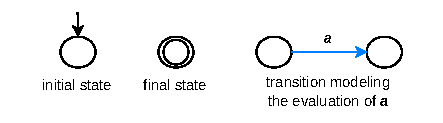
\includegraphics[width=\textwidth]{imgs/GraphicalNotation.pdf}
    \caption{Graphical notation for the representation of FSMs in this document}\label{FSMbase}
\end{figure}

To model the interactions between elements of a chips model, we use the synchronous product with respect to transitions of the interracting FSMs.\\\emph{Insert definition of the synchronous product here}\\ Such operations will be represented in the fashion of Figure~\ref{syncproddef}.

\begin{figure}
    \centering
    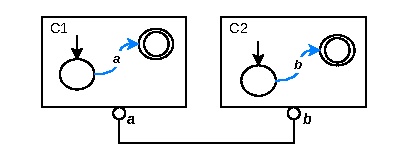
\includegraphics[width=\textwidth]{imgs/SynchronousProductDef.pdf}
    \caption{Graphical notation for the synchronous product of the \emph{C1} FSM and the \emph{C2} FSM w.r.t \emph{a} and  \emph{b} transitions.}\label{syncproddef}
\end{figure}

\subsection*{Writing conventions of this document}

\begin{itemize}
    \item Chips kewords are written in bold font: \textbf{ctx}, \textbf{logical}, \textbf{with}\ldots
    \item Identifiers refer to character strings starting with either a letter (upper or lower case) or the underscore character '\_'. Identifiers only contain alphanumerical characters or underscore characters.
    \item When a given chips element is said to be composed of a \emph{set} of something, there is no order for the elements of the set.
    \item When a given chips element is said to be composed of a \emph{sequence} os something, order of the elements of the sequence matters.
\end{itemize}


\section{Chips code Architecture}

Chips models are distinguished into two sections:
\begin{itemize}
    \item The \emph{preamble} section, which is reseved for the definition of all the model elements,
    \item and the \emph{system} section, which is for instanciating elements and connecting them together to describe a model.
\end{itemize}

Since Chips is based on the concept of functional block models, it allows to describe model elements inner logic as function definitions. This is the main purpose

\section{Preamble content}

\subsection{Definition supertypes}
Chips components fit into three different categories. Each one of these categories represents a different concept in chips models. 

\subsubsection{Functions}
Composed by 
\begin{enumerate}
    \item a name,
    \item a set of input parameters,
    \item a sequence of initializing statements,
    \item a sequence of updating statements,
    \item a set of output expressions.
\end{enumerate}



\subsubsection{Nodes}
Composed by 
\begin{enumerate}
    \item a name,
    \item a sequence of object specific statements (including regular statements).
\end{enumerate}

\paragraph{Node specific statements}
Can be formally described as:
\[
STTS_{node} = STTS_{regular} \cup \{ctx\_decl, channel\_decl\}
\]
where:
\begin{itemize}
    \item[$ctx\_decl$] is the declaration of a variable preceeded by the keyword \textbf{ctx}. We call such variable a \emph{contextual variable}. It is a variable that can be read or written by any functional block linked to the node that declares it.
    \item[$channel\_decl$] is the succession of two identifiers. The first identifier is what we call the \emph{channel type} and the second identifier is tthe \emph{channel name}. The \emph{channel name} identifier then become reserved in the scope of the node statements. Channels are refered to when defining the channel 
\end{itemize}

\subsubsection{Primitive collectives}
Composed by 
\begin{enumerate}
    \item a name,
    \item an accumulator definition,
    \item a node type reference,
    \item a sequence of collective specific statements (including regular statements),
    \item a sequence of updated accumulators,
    \item an output expression.
\end{enumerate}

\subsection{Definition types}
\subsubsection{Logical functions}
\subsubsection{Objects}
\subsubsection{Physical functions}
\subsubsection{Spread}
\subsubsection{Collect}

\section{Statements and expressions}
\subsection{Regular statements and expressions}
\subsection{Collective specific statements and expressions}
\subsection{Object specific statements}


\section{System Description}
\subsection{Variables and constants}
\subsection{Function/Node instanciation}
\subsection{Function feeding}
\subsection{Linking}
\subsection{Regular statements}
\end{document}